\chapter{Incorporation of water-derived hydrogen into
	methane during artificial maturation of kerogen under hydrothermal
	conditions}\label{dx:B}
\chaptermark{Kerogen + D\textsubscript{2}O experiment}



\begin{abstract}

	\noindent To investigate the origin of H in hydrocarbons, particularly methane, we
	reacted a sample of organic-rich Eagle Ford shale with
	D\textsubscript{2}O under hydrothermal conditions in a flexible Au-Ti
	cell hydrothermal apparatus in a water:rock ratio of approximately 5:1.
	Temperatures were increased from 200 to 350~°C over the course of one
	month, maintaining pressure at 350 bar, and the concentrations of
	aqueous species and methane isotopologues produced were quantified.
	Production of H\textsubscript{2}, CO\textsubscript{2}, alkanes, and
	alkenes was observed. Methane formed during the early stages of the
	experiment at 200~°C was primarily CH\textsubscript{4} with some
	CH\textsubscript{3}D, whereas at higher temperatures, increasing
	proportions of deuterated isotopologues were produced, such that near
	the end of the experiment, the concentration of CD\textsubscript{4}
	exceeded that of all other isotopologues combined. These results suggest
	that competition between rates of kerogen-water isotopic exchange and
	natural gas generation may govern the D/H ratio of thermogenic gases.

\end{abstract}

\vspace*{\fill}

\noindent \rule{\textwidth}{0.4pt}\\

{\small
	
	\noindent This appendix contains preliminary results from experimental work
	conducted in collaboration with Jeff Seewald, Eoghan Reeves, and Sean
	Sylva at WHOI with input from Shuhei Ono. \\
	
}

\clearpage


\section{Introduction}\label{introduction-4}

Controls on δD values of thermogenic natural gases are often attributed
to kinetically-controlled fractionation during pyrolysis of kerogen or
oils. There are now several studies which have investigated D/H ratios
of methane and other hydrocarbons as a function of maturity \parencite{Sackett_1978_GCA,Berner++_1995_CG,Sackett+Conkright_1997_GCA,Tang++_2005_GCA,Ni++_2011_GCA}. However, kinetic isotope
effects involving hydrogen addition or abstraction are often large and
by themselves do not explain the geologically-reasonable apparent
equilibrium temperatures of \textasciitilde{}150 to 220~°C obtained for
reservoir gases that have been studied for their clumped isotopologue
compositions \parencite{Stolper++_2014_S,Stolper++_2015_GCA,Wang++_2015_S,Young++_2017_GCA}. There is also evidence that δD values of
CH\textsubscript{4} approach values expected for isotopic equilibrium
between CH\textsubscript{4} and H\textsubscript{2}O in formation waters
at temperatures characterizing reservoirs and/or source rocks
(\textasciitilde{}150 to 250~°C) \parencite{Clayton_2003_IMOG,Wang++_2015_S},
although findings of insignificant hydrogen exchange occurring under
these conditions also exist \parencite{Yeh+Epstein_1981_GCA}. In order for
methane samples to have approached or attained equilibrium values of
Δ\textsuperscript{13}CH\textsubscript{3}D and
Δ\textsuperscript{12}CH\textsubscript{2}D\textsubscript{2}, there must
be a pathway by which either (\emph{i}) isotopes can be exchanged
amongst methane isotopologues alone, (\emph{ii}) methane isotopologues
exchange hydrogen with water or organic molecules, or (\emph{iii})
methane isotopologues are derived from methyl moieties which contain
C--H bonds that have pre-exchanged with water prior to forming methane
\parencite{Hoering_1984_OG,Smith++_1985_OG,Schimmelmann++_1999_GCA,Lis++_2006_OG,Schimmelmann++_2006_AREarth}.

Here, we study the origin of C--H bonds in thermogenic methane by
heating kerogen in the presence of D\textsubscript{2}O, and examining
the degree of deuteration in the generated methane. This experiment is
conceptually very similar to those conducted by \textcite{Hoering_1984_OG,Lewan_1997_GCA,Schimmelmann++_2001_OG}. However, none of these workers
quantified the extent of deuteration in the produced natural gases,
though \textcite{Lewan_1997_GCA} mentioned that methane formed in his experiments
contained deuterium.

\section{Methods}\label{methods-3}

\subsection{Experimental methods}\label{experimental-methods}

Experiments were conducted in a gold-titanium reaction cell housed
within a flexible cell hydrothermal apparatus \parencite{Seyfried++_1987} at
WHOI. The reaction cell was pre-treated prior to loading by an overnight
soak in acid.

A sample of Eagle Ford shale from Uvalde County, Texas, USA was used as the source material for this
experiment. The sample was kindly provided to J. Seewald by Keith F. M. Thompson (PetroSurveys, Inc.), and
was powdered to \textless{}\SI{250}{\micro\meter} and Soxhlet-extracted (by Carl Johnson, WHOI).  After extraction, the rock contained about 11\% total carbon, about half of which is acid-dissolvable carbonate (\autoref{tab:B:EA}). The reaction cell was loaded with 10.03 grams of the Soxhlet-extracted powder.  

The starting fluid in Experiment EF-D2O-1 (``DIPPIE-1'') was heavy water
(D\textsubscript{2}O, 99\% purity, Cambridge Isotope Laboratories, Inc.) containing some NaCl (0.497~mol/kg). The added NaCl allows for detection of dilution of the fluid by deionized water from
the pressure vessel in the case of a leak in the reaction cell. The reaction cell was loaded with 55.03~g of this starting fluid.

\begin{SCtable*}
	\centering
	\caption[Elemental analysis of Eagle Ford shale]{Elemental analysis of Eagle Ford shale powder that was either untreated (UNEX), Soxhlet-extracted (EX), or extracted + decarbonated (DECA).  Data from C.~Johnson, WHOI, 1996.} \label{tab:B:EA}
	\begin{threeparttable}
		\begin{tabular}{c d{3} d{3} d{3}}
			\toprule
			(wt\%)	& \multicolumn{1}{c}{UNEX} & \multicolumn{1}{c}{EX*} & \multicolumn{1}{c}{DECA} \\
			\midrule
			C & 12.1  & 11.0 & 6.23 \\
			H & 0.38  & 0.25 & 1.24 \\
			N & 0.18  & 0.17 & 0.74 \\
			S & 0.37  & \textless\!\!0.2 & 2.3  \\
			\bottomrule
		\end{tabular}
		\begin{tablenotes}
			\item * Used in the experiment.
		\end{tablenotes}
	\end{threeparttable}
\end{SCtable*}


\subsection{Analytical methods}\label{analytical-methods}

To monitor the fluid composition and the extent of deuteration, samples
aliquots of fluid were withdrawn through the capillary exit tube into
gastight glass/PTFE syringes. Immediately prior to a sampling event, a
small amount (\textasciitilde{}0.5 g) of fluid was removed and discarded
in order to flush the exit tube of any residues.

The concentration of molecular hydrogen (H\textsubscript{2}) was
determined after headspace extraction using a gas chromatograph supplied
with nitrogen carrier gas, and equipped with a molecular sieve 5Å column
and thermal conductivity detector. Analytical reproducibility of
H\textsubscript{2} data is ±10\% or better (2\emph{s}), however,
accuracy of reported concentrations is currently unknown, because the
relative response of H\textsubscript{2} and D\textsubscript{2} (likely
to be the main form of molecular hydrogen) in the GC-TCD has not yet
been determined. Residual liquid after headspace extraction was diluted
with MilliQ water and saved for analysis of major cations and anions, or
stored with dichloromethane in the fridge in a screw capped vial for
analysis of non-volatile organic compounds.

Concentrations of total dissolved inorganic carbon
($\big\sum\!$CO\textsubscript{2}) and C\textsubscript{1} to C\textsubscript{6}
alkanes and alkenes were determined using a purge-and-trap cryofocusing
device coupled to a gas chromatograph equipped with a Porapak Q column
and serially-connected thermal conductivity and flame ionization
detectors. Analytical procedures were as described in \textcite{Reeves++_2012_GCA}}. Analytical reproducibility on duplicate samples was ±5\% or
better (2\emph{s}). The C\textsubscript{5} and C\textsubscript{6}
compounds could not be quantified accurately due to their semi-volatile
nature; however, C\textsubscript{5} and C\textsubscript{6} were detected
at all sampling points.

At each sampling, a separate \textasciitilde{}1 to 2~ml aliquot was
injected directly into a pre-weighed, evacuated serum vial capped with
boiled blue butyl rubber stoppers, for analysis of the extent of
deuteration of methane. A Hewlett-Packard (HP) 6890 gas chromatography-mass
spectrometry (GC-MS) system equipped with a 5Å molecular sieve column (HP-PLOT 30 m $\times$ 0.32 mm $\times$ \SI{12.0}{\micro\meter}) and HP 5973 mass selective detector was
used to determine the amount of deuteration in CH\textsubscript{4}. Ion
currents were monitored at integral masses between \emph{m}/\emph{z} 10 and 50. Extracted ion currents were quantified at \emph{m}/\emph{z} 14 through 23 for methane.  Expected fragmentation patterns of each of the methane-\emph{d} isotopologues were determined by analysis of commercial synthetic standards (\textgreater{}98\% purity, Cambridge Isotope Laboratories, Inc.).

\section{Results \& Discussion}\label{results-discussion-1}

\subsection{Concentrations of aqueous
	species}\label{concentrations-of-aqueous-species}


\begin{sidewaysfigure}
	\centering
	\includegraphics[width=\textwidth]{figures/FigB.1}
	\caption[Concentrations of aqueous species during experiment EF-D2O-1.]{Concentrations of aqueous species during experiment EF-D2O-1.  Note the log scale for concentration.}
	\label{fig:B:1}
\end{sidewaysfigure}

\begin{sidewaysfigure}
	\centering
	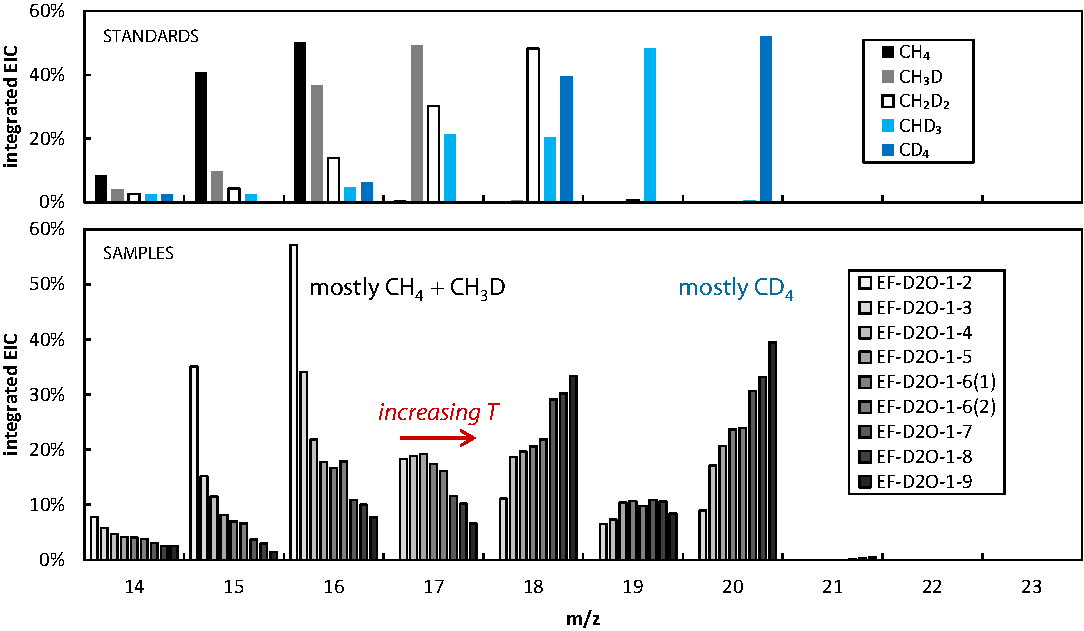
\includegraphics[width=0.85\linewidth]{figures/FigB.2}
	\caption[Mass spectra of methane generated in experiment EF-D2O-1]{Mass spectra of methane generated from artificial maturation of Eagle Ford shale in the presence of D\textsubscript{2}O.}
	\label{fig:B:2}
\end{sidewaysfigure}

\begin{SCfigure*}
	\centering
	\includegraphics[width=0.75\linewidth]{figures/FigB.3}
	\caption[Estimated relative and absolute abundances of methane
	isotopologues in experiment EF-D2O-1]{Estimated relative and absolute abundances of methane
		isotopologues. Concentrations less than zero are an artifact of
		uncertainty in standardization and may potentially be corrected by
		applying algorithms to account for contributions of fragment ions to
		peaks in the lower range of \emph{m}/\emph{z}. Note the log scale on the \emph{y}-axis in the
		bottom panel.}
	\label{fig:B:3}
\end{SCfigure*}
\begin{table*}
	\centering
	\caption[Concentration of aqueous species during Experiment	EF-D2O-1]{Concentration of aqueous species during Experiment EF-D2O-1, heating of Soxhlet-extracted Eagle Ford shale at 200 to 350~°C	and 350~bar in the presence of saline D\textsubscript{2}O fluid.}
	\label{tab:B:1}
	\begin{threeparttable}
		\begin{tabular}{c c ccc c c}
			\toprule
			Sample	& Time 	& \ce{H2} 	& \ce{CH4}	&  $\big\sum\!$\ce{CO2} 	& \multirow{2}{*}{C\textsubscript{1}/C\textsubscript{2--4}}	& pD\\%\tnote{a} \\ 
			\# 		&  (h)	& (µmol/kg) & (µmol/kg) & (mmol/kg)	& & (25~°C)\\
			\midrule
			\multicolumn{7}{l}{\emph{Experiment begun with 52.6 g fluid at temperature of 200~°C}}\\
			1 &	19	& BDL (\textless{}10) &	1.2	& 4.8 &	0.11&\\	
			2 &	164	& BDL (\textless{}10) &	3.8 &	10.8 &	0.37&\\	
			\multicolumn{7}{l}{\emph{Temperature raised to 300~°C}}\tabularnewline
			3 &	191	& 773 &	87	& 21.9 &	1.00	&\\
			4 &	284	& 183 &	235	& 45.8 &	0.86	&\\
			5 &	427	& 290 &	396	& 65.5 &	0.86	&\\
			\multicolumn{7}{l}{\emph{Injected \textasciitilde{}18.3 g starting fluid and raised temperature to 325~°C}}\tabularnewline
			6 &	451	& 353 &	319	& 44.7 &	0.89	&\\
			7 &	598 & 586 &	825	& 45.3 &	0.85	&\\
			\multicolumn{7}{l}{\emph{Raised temperature to 350~°C}}\tabularnewline
			8 &	617	& 718 &	$ 1.32\times10^3 $ &	54.4 &	0.89 &	\\
			9 &	836	& 821 &	$ 3.47\times10^3 $ &	51.2 &	1.00 &	5.90\\
			\bottomrule
		\end{tabular}
	
		\begin{tablenotes}
			\item[a] The listed pD value was calculated from pH measured
			with a glass electrode: pD = pH\textsubscript{measured} + 0.41 \parencite{Glasoe+Long_1960_JPC}.
		\end{tablenotes}
	\end{threeparttable}
\end{table*}
%\multirow{2}{*}{C\textsubscript{1}/C\textsubscript{2--4}}

%\begin{table}
%	\begin{tabular}{c c c}
%		AAA & 1 & 22\\
%		BBB & 2 & 33\\
%	\end{tabular}
%\end{table}

Measured concentrations of aqueous species are shown in \autoref{fig:B:1}.
Concentrations of H\textsubscript{2} increased from undetectable
(\textless{}10~µmol/kg) to up to 0.8~mmol/kg at the end of the
experiment. Increasing concentrations of H\textsubscript{2} within
temperature stages of the experiment suggests that generation of
petroleum, as opposed to a mineral redox buffer, is influencing the
H\textsubscript{2} concentration. H\textsubscript{2} increased much more
slowly during the \textgreater{}300~°C stages compared to heating at 300~°C and below.

The concentration of $\big\sum\!$CO\textsubscript{2} increased during the early
stages of the experiment, and leveled off at \textasciitilde{}50~mmol/kg
at 350~°C. This might indicate that carbonate reached saturation and began to precipitate
\parencite{Seewald++_1998_GCA}; to verify this, measurements of major cations
are required. Production of CO\textsubscript{2} as the most abundant
product of hydrothermal alteration of kerogen is also consistent with
prior experimental work \parencite{Seewald_2003_N}. Alternatively, carbonate could have been released from the rock as it had not been decalcified prior to heating. 

Concentrations of methane
increased at all time steps, as did concentrations of detected
\emph{n}-alkanes. Except for the beginning of the experiment, molar
concentrations of C\textsubscript{1} and $\big\sum\!$C\textsubscript{2--4} were
very similar and increased in near lock step.

\subsection{Production of deuterated
	methane}\label{production-of-deuterated-methane}



The relative abundance of methane-\emph{d} isotopologues was quantified by GC-MS
for all samples except the one from timepoint \#1, for which no methane
peaks of usable size could be obtained (\autoref{fig:B:2}).

Methane formed during the early stages of the experiment at 200~°C was
primarily CH\textsubscript{4} with some CH\textsubscript{3}D, whereas at
higher temperatures, the isotopologues produced consist almost
exclusively of CD\textsubscript{4}, CH\textsubscript{3}D, and
CH\textsubscript{2}D\textsubscript{2} (\autoref{fig:B:3}). These results suggest
that at relatively lower temperatures of \textasciitilde{}200~°C, the
rate of methane generation approaches or exceeds the rate of D/H
exchange between water and kerogen, whereas at higher temperatures,
extensive D/H exchange between kerogen (or oils, if they are also
precursors of methane) and water occurs prior to methane generation.
CD\textsubscript{4} became the dominant methane species at temperatures
of 300~°C and above, suggesting that more than 50\% of all labile,
methane-generating sites on kerogen were fully deuterated.
Alternatively, the dominance of CD\textsubscript{4} might be explained
by direct CH\textsubscript{4}--H\textsubscript{2}O isotopic exchange
occurring after the generation of primarily non-deuterated methane. This
is unlikely given the sluggish pace at which D/H exchange occurs for
methane \parencite{Reeves++_2012_GCA}. Experiments in which normal water is
heated in the presence of CD\textsubscript{4} while the D/H of water is
monitored may yield a more sensitive determination of the exchange rate
constant for CH\textsubscript{4}--H\textsubscript{2}O.

Production of CH\textsubscript{4} at the beginning of the experimenst
indicates that the ``capping'' hydrogen was derived from kerogen or
other H-containing species in the rock as opposed to water.
Alternatively, the CH\textsubscript{4} observed at the first time point
may have been sorbed to a solid phase and leached into the fluid.
Production of CH\textsubscript{4} and CH\textsubscript{3}D appeared to
cease by midway through the 300~°C stage. Continued (though relatively
minor) production of methane that was not fully-deuterated
(CHD\textsubscript{3} and CH\textsubscript{2}D\textsubscript{2}, \autoref{fig:B:3},
bottom panel) suggests that kerogen or oil from which methane was
generated did not fully exchange before methane formed.

While examining the total ion and extracted ion chromatograms to
quantify the deuteration in CH\textsubscript{4}, an unknown and
unexpected peak was found eluting immediately following the
CH\textsubscript{4} and air peaks. This mystery peak appeared to yield
methyl fragments that were also progressively more deuterated with
reaction time. Re-analysis of several samples while scanning a higher
mass range suggested that the mystery compound had stable fragments near
\emph{m}/\emph{z} 45 to 50 (depending on degree of deuterium
substitution). This was verified by GC-MS analysis of a commercial
isobutane standard (mostly isobutane-\textit{d}\textsubscript{0}) which yielded a
base peak at \emph{m}/\emph{z} 43. No attempt to quantify the degree of
deuteration in isobutane was made.

\section{Acknowledgments}\label{acknowledgments-4}

Financial support for this work was provided by a Shell-MITEI Fellowship
and by NSF award EAR-1250394 to S. Ono.




